\documentclass[11pt]{amsart}
\usepackage{geometry}                % See geometry.pdf to learn the layout options. There are lots.
\geometry{letterpaper}                   % ... or a4paper or a5paper or ... 
%\geometry{landscape}                % Activate for for rotated page geometry
\usepackage[parfill]{parskip}    % Activate to begin paragraphs with an empty line rather than an indent
\usepackage{graphicx}
\usepackage{amssymb}
\usepackage{epstopdf}
\usepackage{natbib}
\DeclareGraphicsRule{.tif}{png}{.png}{`convert #1 `dirname #1`/`basename #1 .tif`.png}

\title[Lamarck]{Lamarck:\\Modelling ecological communities as if they were DNA}
\author{William D. Pearse}
\date{\today}                                           % Activate to display a given date or no date
\begin{document}
\bibliographystyle{besjournals}
\maketitle
\section{Abstract}
\clearpage
\section{Introduction}
Many ecologists are interested in how the composition of communities changes over time, and are interested in competition between species. However, modelling such changes over time is difficult. Modelling the population numbers of individual species within a community is difficult, because there are often so many different species in a community that too many parameters would need to be estimated. Conversely, while summary statistics can give insight into the general structure of a community, a single uni-dimensional measure cannot capture the complexity of a system, and it is hard to make meaingful species-level predictions using them.

One way round this problem has been to model a community as proceeding through a series of states, each with their own associated species compositions and abundances. The probability of moving through between these states can be modelled using Markov Chains, and thus meaningful predictions can be made. However, such methods require \emph{a priori} definitions of states, ignore the continuous turnover within the states we are interested in, assume the history of a community is unimportant, and require that the system reaches a final, stable state \cite{Logofet2000}.

My alternative is to model species turnover as a transition matrix, where the likelihood of a species entering a community can be predicted by the identity of the species they replace. The problem is then analogous to parameterising a substitution model when building a phylogeny from DNA data. Simplifying the transition matrix in the same way we search for the optimal substitution model could help identify `important' species transitions.
\clearpage
\section{Methods}
\subsection{Description of Method}
\subsection{Simulation Data}
To check the method worked on what might be considered ideal data, two main kinds of random datasets were produced. In each, the number of species, communities, years, number of starting individuals and number of individuals added each year were varied (see table X). In the first, all species had essentially the same parameters. In the other each species had a randomly selected `stable' parameter and another transition parameter estimated such that the two summed to 0.8, and the other parameters evenly distributed. The `addition' parameters were also randomly chosen. Examples of both are shown in table X.

Each simulation's results were compared with the parameters used to generate them using Mantel tests, and the resulting $r^{2}$ values recorded. Mantel tests are often conservative, and so considered safe for the present purpose.
\subsection{Ecological Data}
Butterfly community data were taken from the UK Butterfly Monitoring Scheme (UKBMS), a scheme that has repeatedly-sampled butterfly community data dating back to 1974. The 100 best-recorded sites' yearly species abundances were taken and used as input data for the program. All of the data from all of the communities were fitted simultaneously, fitting both the maximal model and the stepwise-addition method.

Once these estimates had been generated, the transitions parameters were compared (using a phylogenetic Mantel test) with a previously-generated phylogeny of all butterflies in the UKBMS scheme (figure Y). In brief, this phylogeny (\ref{phylogeny}) was generated using the cytochrome oxidase one gene and BEAST \citep{Drummond2006,Drummond2007,Drummond2012}, with some constraints fitted above family level as described in its legend. Pagel's $\lambda$ values were calculated for the addition parameters. Both of these tests would show whether the interactions of the species were phylogenetically conserved, which would be in keeping with other (unpublished) work by the author on this dataset.
\begin{figure}
\begin{center}
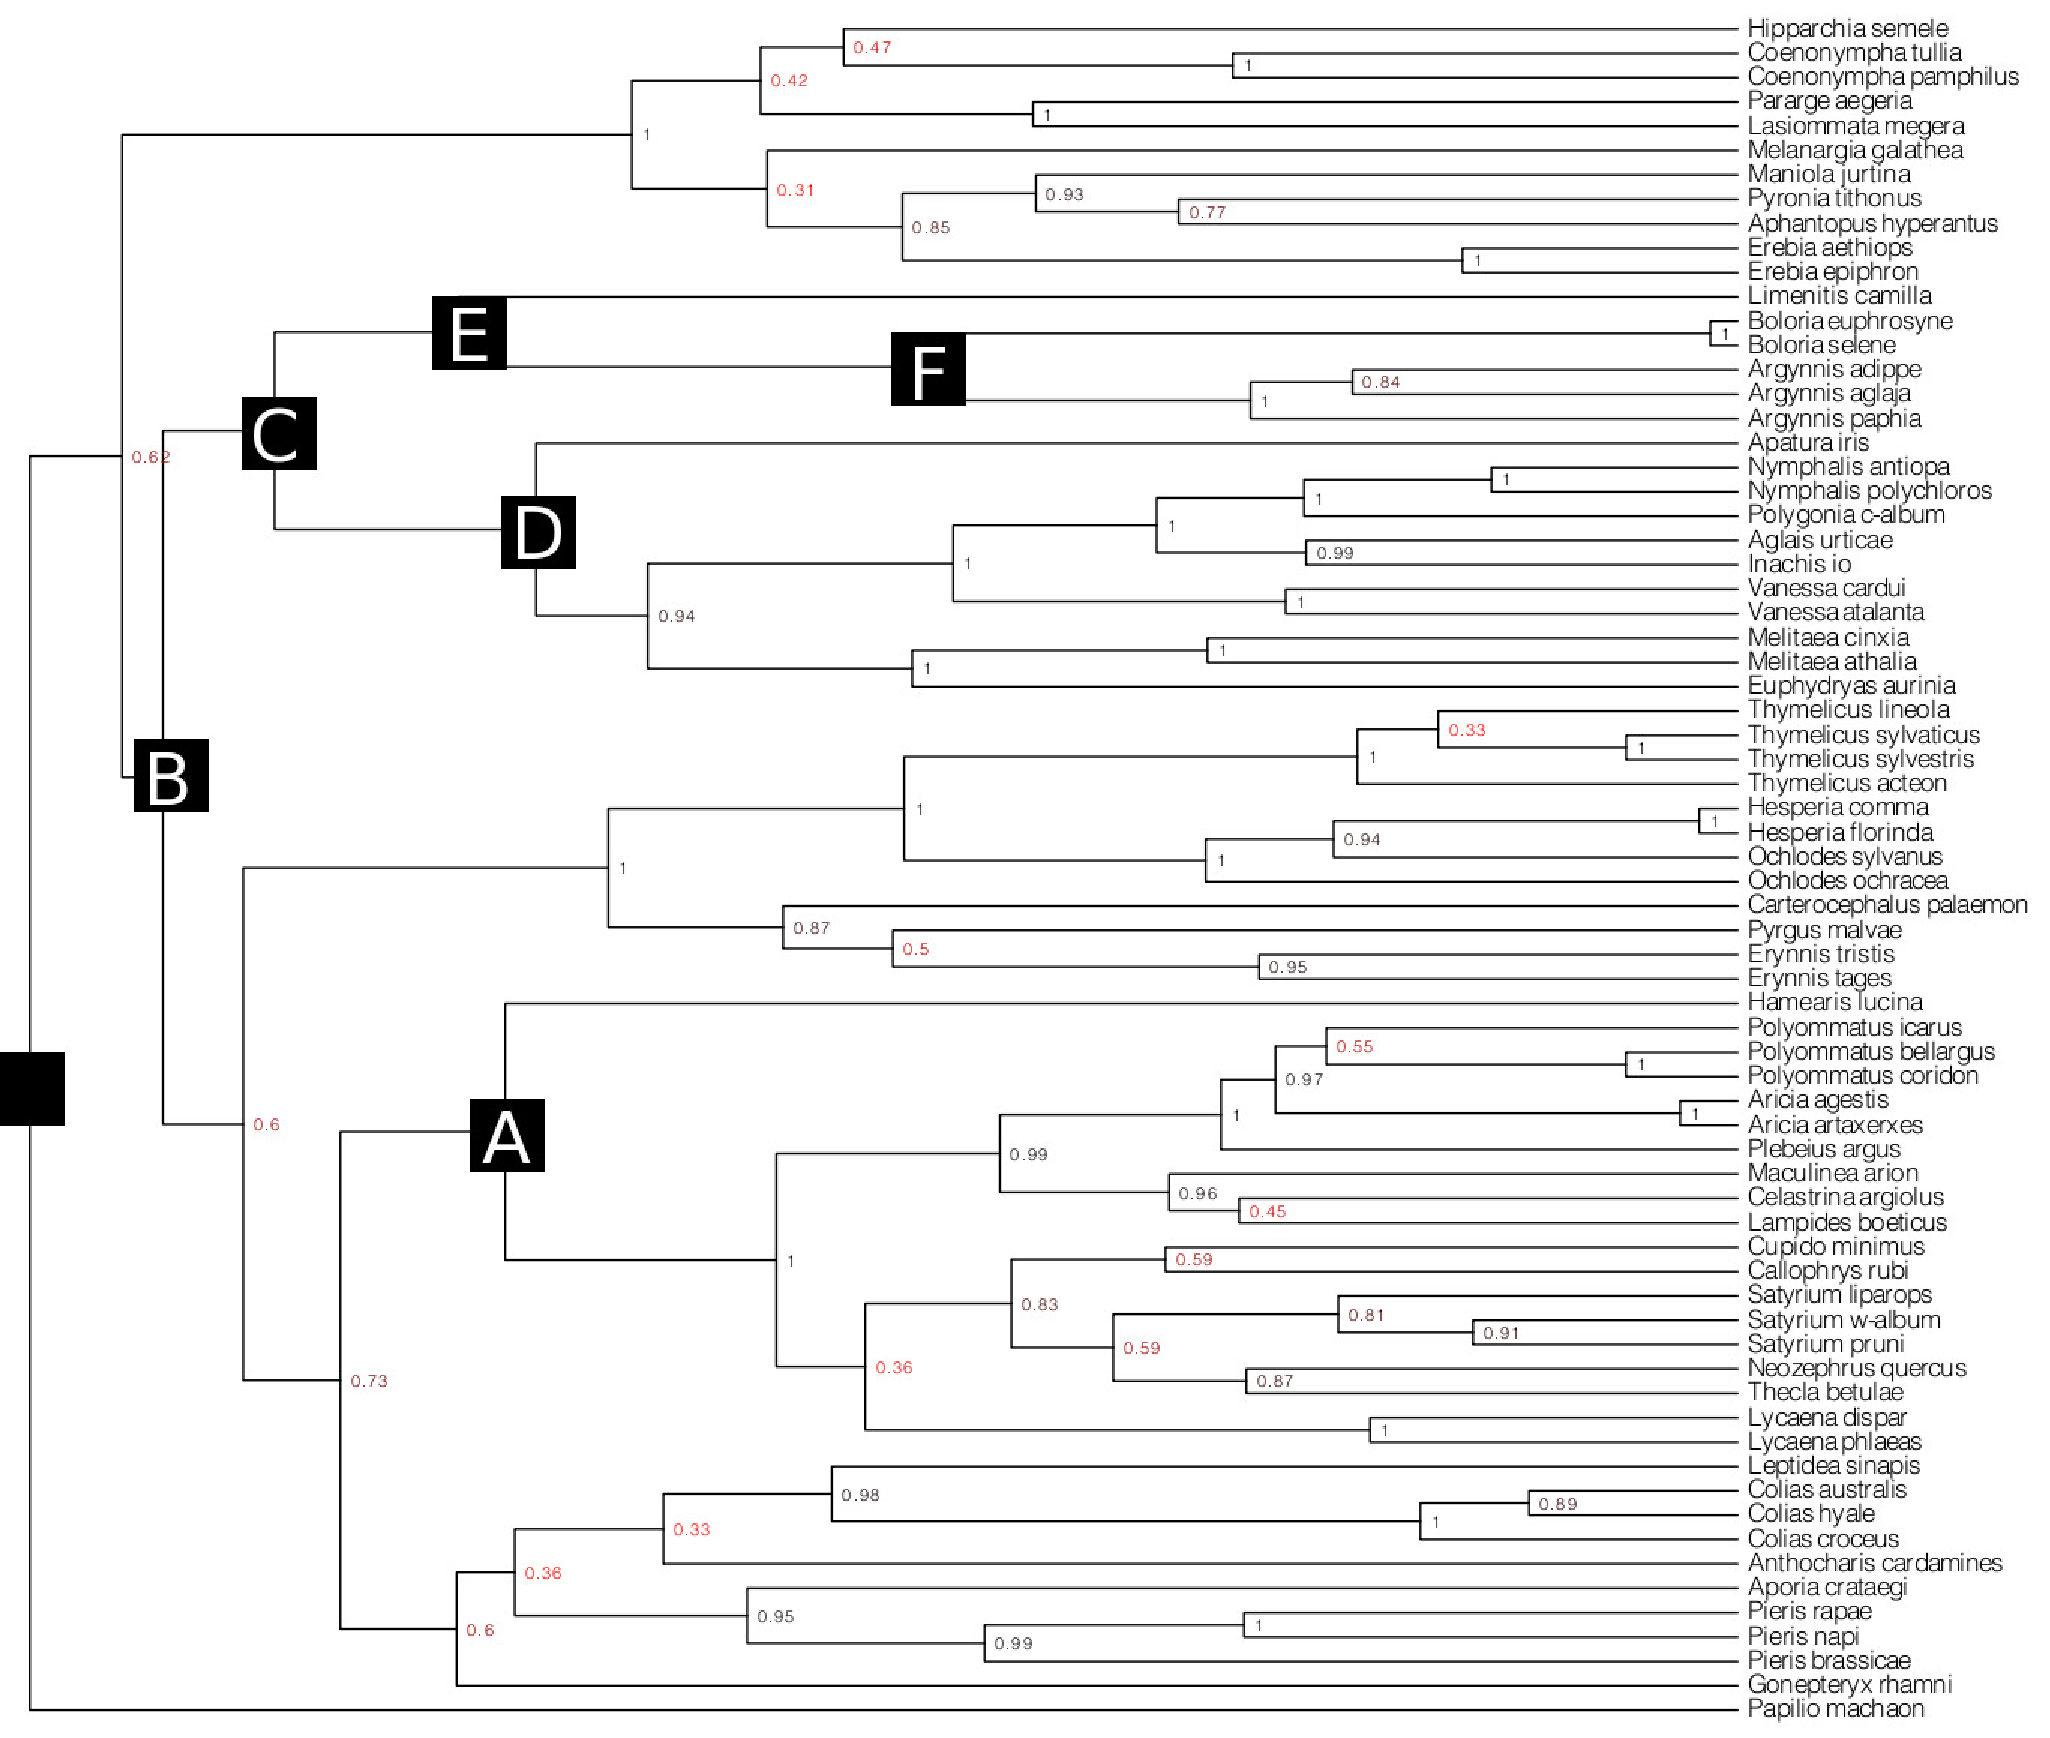
\includegraphics[width=\textwidth]{phylogeny}
\caption[Butterfly phylogeny.]{Butterfly phylogeny. Letters at nodes indicate clades that were constrained to be monophyletic based on recent multi-locus higher-level Lepidoptera phylogenies (A, C, D, E, E --- \citet{Wahlberg2010} and B --- \citet{Mutanen2010}). Numbers at nodes indicate posterior probabilities; the more read a number, the less support there is for that node.}
\label{phylogeny}
\end{center}
\end{figure}
\clearpage
\section{Results}
\subsection{Simulation Data}
\subsection{Ecological Data}
\clearpage
\section{Discussion}
\subsection{Biological Interpretation}
\subsection{Method Performance and Future Directions}
\clearpage
\section{Acknowledgements}
\clearpage
\bibliography{Library}
\end{document}  